\chapter{Semi-Statistical Study of Dimming-CME Relationship}
\label{chapterstatistical}

% Mini-abstract
Extreme ultraviolet (EUV) coronal dimmings are often observed in response to solar eruptive events. These phenomena can be generated via several different physical processes (see Chapter \ref{chaptermechanisms}). For space weather, the most important of these is the temporary void left behind by a coronal mass ejection (CME). Massive, fast CMEs tend to leave behind a darker void that also usually corresponds to minimum irradiance for the cooler coronal emissions. If the dimming is associated with a solar flare, as is often the case, the flare component of the dimming in the cooler coronal emission can be isolated and removed from the dimming light curve using simultaneous measurements of warmer coronal lines (see Chapter \ref{chaptercasestudy}). In the present Chapter, we apply this technique to 38 dimming events: the two case studies from Chapter \ref{chaptercasestudy} plus 36 additional events taken from two separate two-week periods in 2011. Dimming is then parameterized in terms of depth and slope for each of the events. We provide statistics on which combination of wavelengths worked best for the correction method, describe the fitting methods applied to the dimming light curves, and compare the dimming parameters with corresponding CME parameters of mass and speed. The best linear relationships found with an accuracy of about 20\% are that the CME speed is about 630 km/s times the dimming slope ($\%\ hour^{-1}$) and the CME mass is about $1.03 \times 10^{15}\ g$ times the dimming depth (\%). These relationships could be used for space weather operations of estimating CME mass and speed using near-realtime irradiance dimming measurements.

\section{Introduction to Dimming and CME Parameterization and Statistics}
Extensive surveys of coronal dimming events and their relation to CMEs have been performed by \citet{Reinard2008, Reinard2009}. For their sample of ~100 dimming events, \citet{Reinard2008} found mean lifetimes of 8 hours, with most disappearing within a day. \citet{Reinard2009} studied CMEs with and without associated dimmings, finding that those with dimmings tended to be faster and more energetic. \citet{Bewsher2008} found a 55\% association rate of dimming events with CMEs, and conversely that 84\% of CME events exhibited dimming. The timescale for dimming development is typically several minutes to an hour. This is much faster than the radiative cooling time, which implies that the cause of the decreased emission is more dependent on density decrease than temperature change \citep{Hudson1996}. Dimming regions occur on a spatial scale similar to CMEs, more so than other CME-associated activity (such as flares and EUV waves). Studies have demonstrated that dimming regions can be a good indicator of the apparent base of the white light CME \citep{Thompson2000, Harrison2003, Zhukov2004}. Thus, dimmings are usually interpreted as mass depletions due to the loss or rapid expansion of the overlying corona \citep{Hudson1998, Harrison2000, Zhukov2004}. Spectroscopic observations of coronal dimmings \citep{Harra2001, Harrison2003, Harra2007} found blueshifts in several coronal lines, indicating outflow in dimming regions. Dimmings have also been shown to extend deep into the corona and possibly the chromosphere and photosphere \citep{McIntosh2007}. When dimmings are present with a CME, they are one of the earliest signatures of the actual mass ejected from the low corona, and provide unique information on the onset time and location of the ejection. Many landmark studies have established that dimmings can contribute a large fraction of the mass to a CME \citep{Harrison2000, Harrison2003, Zhukov2004, Aschwanden2009}. There are well-established methods to derive the mass properties of CMEs, but there are still outstanding questions involving the source of the CME mass: how much of the mass comes directly from the erupting region, how much comes from the surrounding or overlying large-scale corona, and how much is "swept up" as the CME propagates \citep{Bein2013}.

An Earth-directed CME’s potential geoeffectiveness is typically characterized by three values: its velocity, mass, and the magnitude and duration of the southward component of the magnetic field ($B_z$) impacting Earth. Typical CME forecasts provide a predicted Earth arrival time only. The geomagnetic storm magnitude is strongly linked to the CME momentum and magnetic field orientation while arrival time at Earth is primarily dependent on CME velocity. The current standard process for estimating velocity relies on sequential coronagraph images from SOHO/LASCO and STEREO/SECCHI. There are ground-based white light coronagraph measurements, such as by High Altitude Observatory’s K-Cor instrument, but those measurements are limited to the low corona and constrained by the times that the Sun is at a sufficiently high elevation as viewed from a fixed-position on Earth’s surface (typically $<$6 hours/day). Analysis of coronagraph images to determine CME velocities and masses results in relatively large uncertainties of 30-50\% \citep{Vourlidas2000, Vourlidas2010, Vourlidas2011}. The velocity and mass measurements with the most uncertainty are for Earth-directed CMEs that are seen as halos in coronagraphs at or near Earth. For these CMEs, a velocity is significantly affected by projection on the plane-of-sky, and a large percentage of the mass can be hidden behind the instrument’s occulter. Without observations of these CMEs from another viewpoint, such as STEREO, it is difficult to make an accurate measurement of the CME velocity and mass from the coronagraph observations. However, dimmings associated with these CMEs are very well observed by Earth-based observations. Our studies of coronal dimming events have focused on the possibility of coronal dimming observations providing useful indicators for CME velocity and mass, and can readily be combined with most $B_z$ prediction methods.

While earlier studies showed that dimmings can account for a significant fraction of the mass ejected, multi-viewpoint observations using STEREO data have the advantage of providing independent mass measurements for the same event from two different aspect angles, yielding a better mass accuracy. In a survey of six STEREO events observed as dimming by EUVI and as CMEs by COR2, \citet{Aschwanden2009} found a clear correspondence between the EUV and white light mass estimates. \citet{Colaninno2009} developed a ‘triangulation’ method to estimate the true (accurate) mass of CMEs from SECCHI observations. More recently, \citet{Bein2013} applied similar methods to a larger CME sample (25 events) and over an extended height range, allowing them to remove the effects of the CME emerging from behind the occulter and to calculate the mass flux of the CMEs in the lower corona.

Standard plane-of-sky velocity estimates are made and cataloged by the Coordinated Data Analysis Workshops (CDAW) CME catalog \citep{Gopalswamy2009}, which use routinely produced SOHO/LASCO coronagraph images. The different views from LASCO and SECCHI images can be used to better constrain the velocity, direction, and mass of CMEs (e.g., \citealt{Colaninno2009}). None of these methods can be used to estimate $B_z$ but velocity is of particular use to space weather forecasters for predicting Earth-arrival times.

In the present chapter, we analyze 38 coronal dimming events -- the two from Chapter \ref{chaptercasestudy} plus 36 more during two separate two-week periods during 2011 -- and search for the relationship between dimming and CME velocity and mass. Of the events studied, 17 could be parameterized in both dimming with EVE data and CME velocity from LASCO and SECCHI observations, and 14 events in dimming with EVE data and CME mass from the coronagraph observations. 

Section \ref{sec:eventselection} shows some examples of observations and describes the method for selecting this sample of events and explains why some events identified in AIA could not be analyzed with EVE and/or SECCHI. Section \ref{sec:deconvolutionstatistics} provides examples and statistics on the flare-peak correction method detailed in Section \ref{sec:deconvolve}, specifically which combinations of dimming and non-dimming lines provided the best correction for each of the events. Section \ref{sec:fittingmethod} describes the fitting method applied to the deconvolved EVE light curves, including a discussion of uncertainties. Finally, Section \ref{sec:correlation} shows the correlations between the various combinations of coronal dimming and CME parameters, and conclusions about dimming and CME relationships are presented in Section \ref{sec:chapter5summary}.

\section{Observations and Event Selection}
\label{sec:eventselection}
In addition to the two cases studied in detail (see Chapter \ref{chaptercasestudy}), four weeks were selected in 2011 for analysis of coronal dimming events: February 10-24 and August 1-14 (Figure \ref{fig:historicalcontext}). These two independent periods about 6 months apart were chosen as appropriate times during the initial rise of solar activity during solar cycle 24. The initial criterion for this selection is to have a total period of time that could result in more than 30 identifiable events. It is also desirable to select a time when the two STEREO spacecraft orbital locations were advantageous for geometric analysis, and when the other space-based instruments used in this study could be expected to be operating nominally. The periods of study are typical in terms of CME occurrence and solar EUV irradiance variability, both near their mean values (see Figure \ref{fig:historicalcontext}).
 
\begin{figure}[!h]
    \begin{center}
	    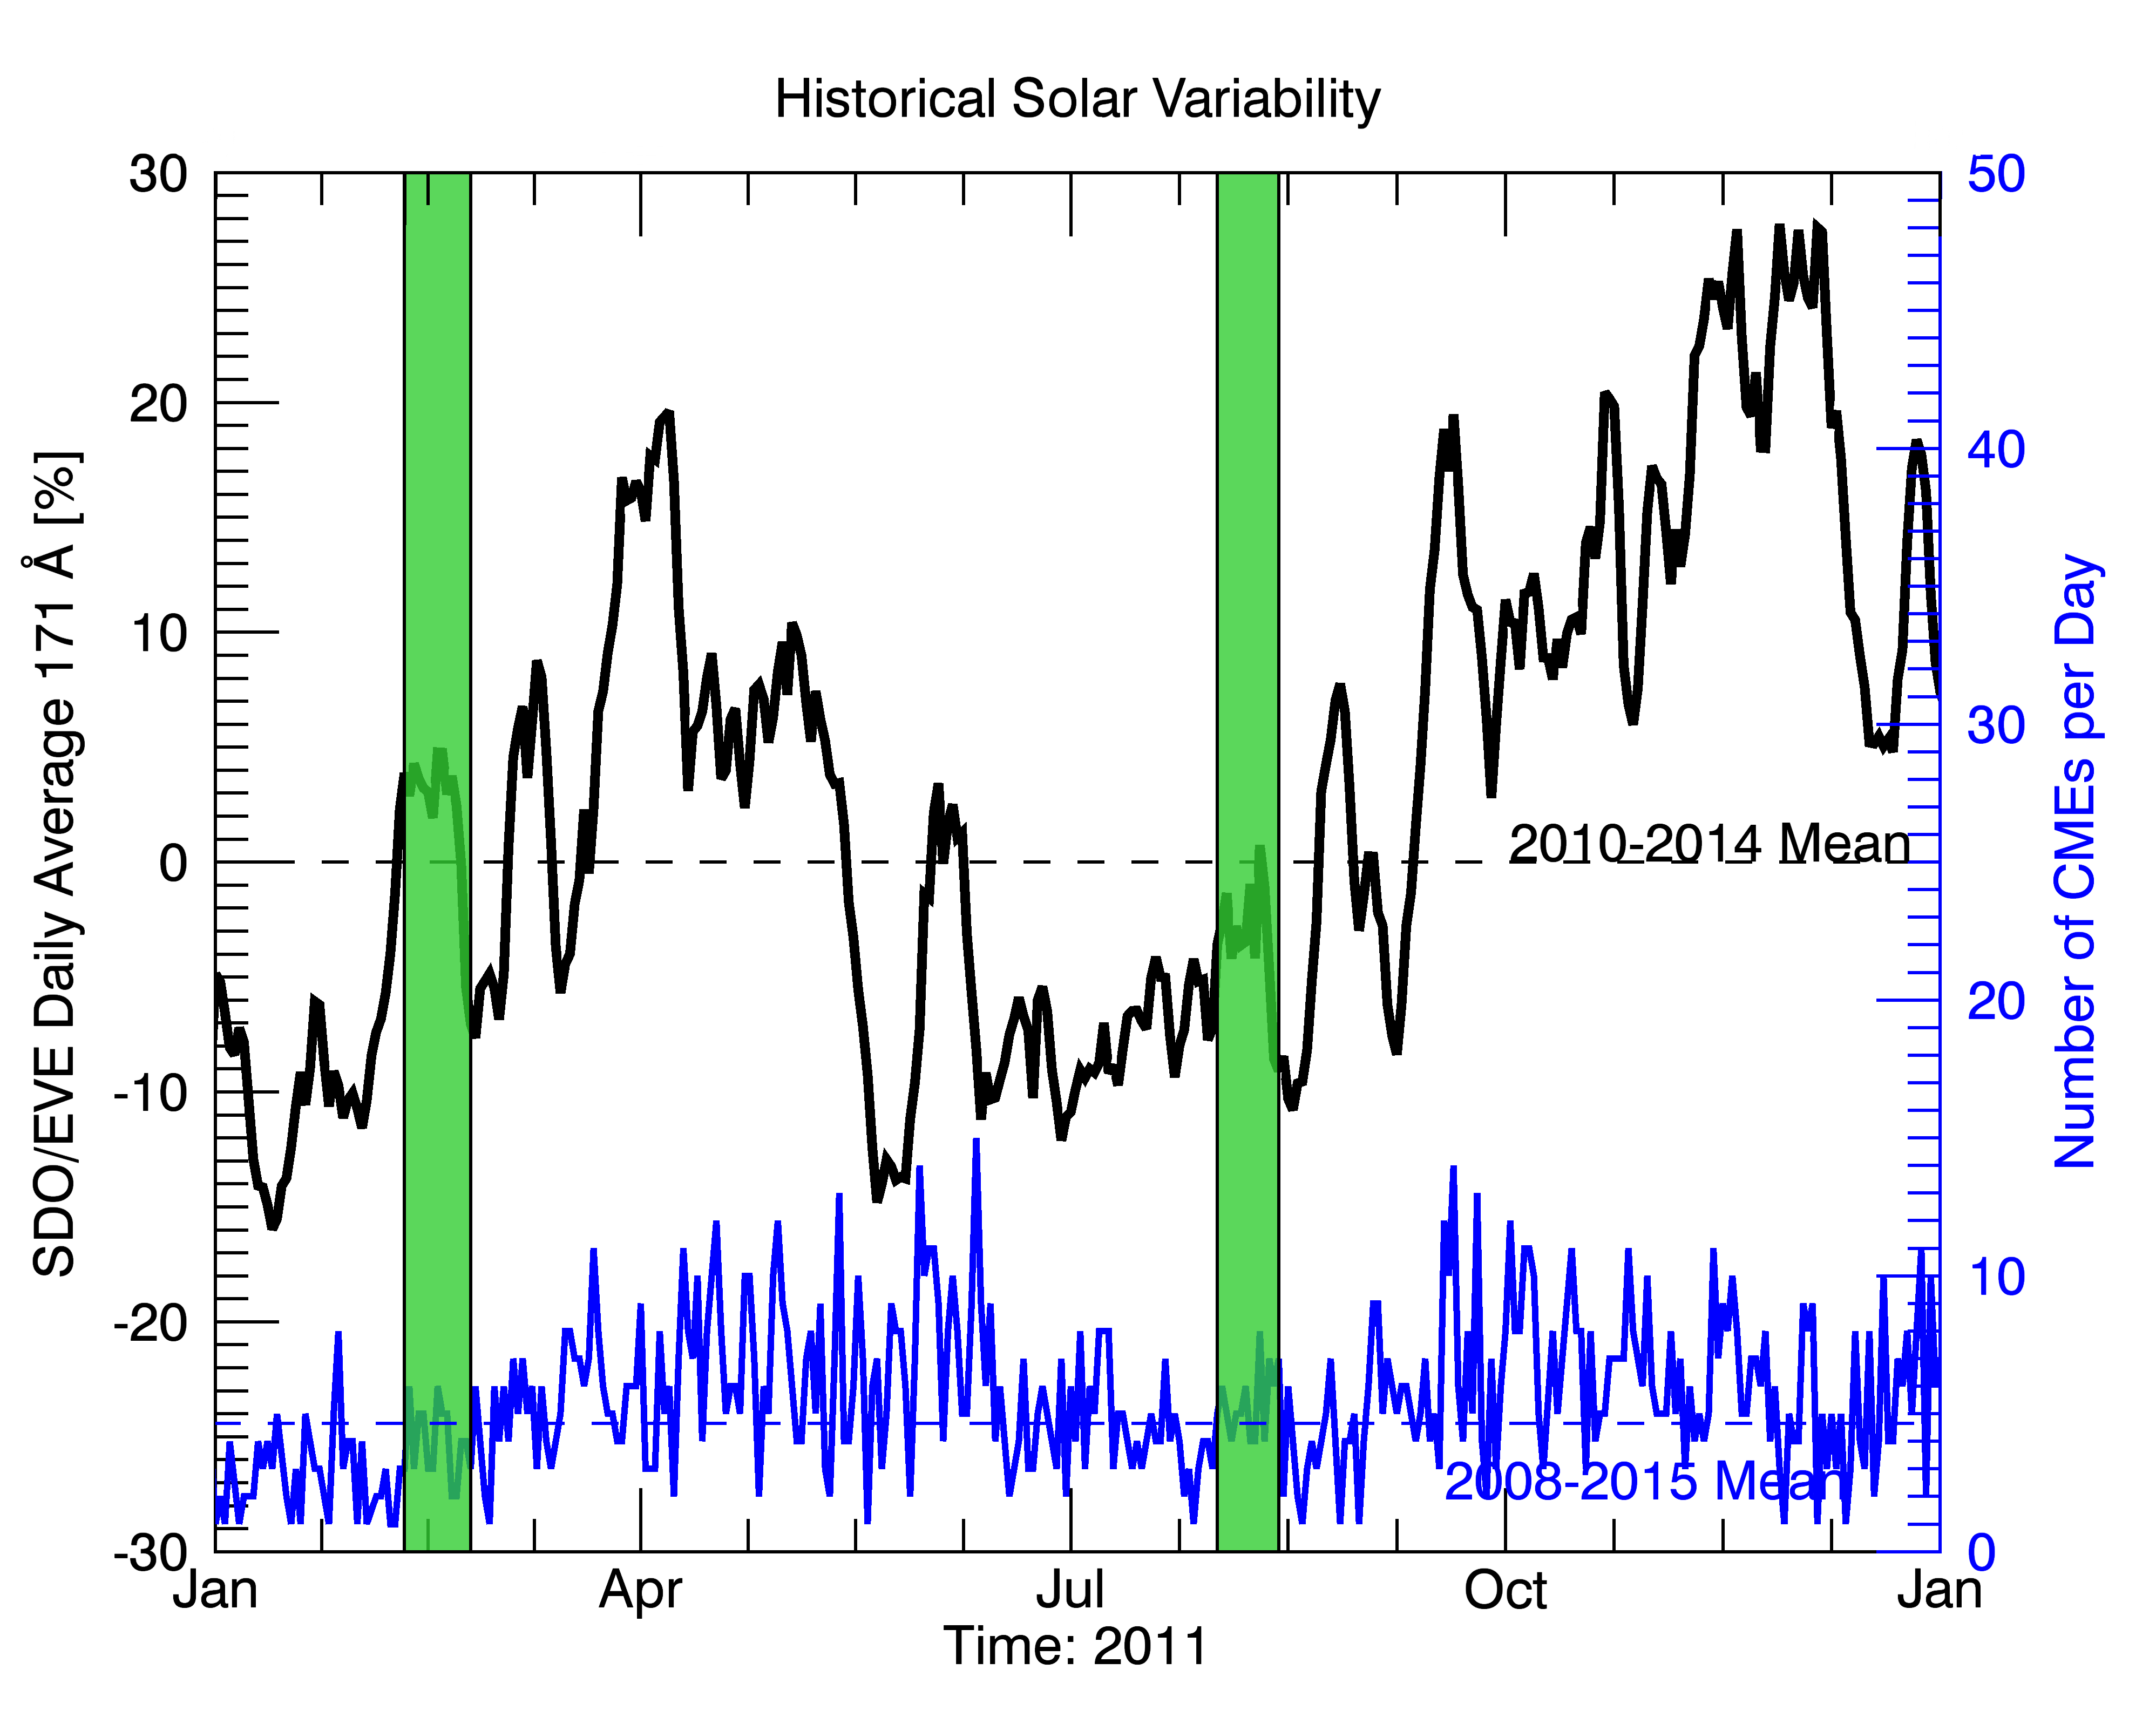
\includegraphics[width=150mm]{Images/FourWeekContext.png}
    \end{center}
    \caption[Selected four week period in historical context]{
        Context for the selected periods of study. The black line is the daily averaged EVE Fe IX 171 \AA\ line and the 
        blue line is the daily total CME occurrence. The vertical green bars indicate the selected periods of this study.
        The mean for EVE (dashed black line) is taken over the first four years of EVE's operations (2010-2014) and the 
        mean for CME occurrence (dashed blue line) is taken for the most recent solar cycle starting in 2008 to the present 
        date.
	}
    \label{fig:historicalcontext}
\end{figure}
 
Images from AIA were used to first identify dimming events. Identification was performed manually using daily AIA movies to create a list of candidate events. Two people made the identifications separately, looking at different movies. James Mason used the AIA 211-193-171 \AA\ composite movies (e.g., Figure \ref{aiacomposite2010aug7}) and Dave Webb used the 193 \AA\ movies. The primary initial selection criteria were that 1) the dimming must persist for several hours and 2) the dimming have non-trivial spatial extent e.g., at least comparable to the size of an active region. The independently identified events were then accumulated, duplicates merged as positively identified events, and disparities investigated by each identifier. Sometimes disparities proved to be questionable events according to the selection criteria above and were removed from the event list. Other times the disparities proved that the independent analysis acted as a failsafe -- a single observer simply missed an event but the other caught it. Future studies will use the automated AIA dimming detection method developed by \citet{Krista2013a}. 
 
Once the event list was deconflicted, the approximate time of the event was used to search the related observations in other instruments: flares from GOES X-ray flux, CMEs from LASCO and COR, and solar irradiance from EVE. This initial list included 38 events (includingw the 2010 August 7 simple case from Chapter \ref{chaptercasestudy}, which was outside the four week period). In some cases, the dimming was not clear in EVE data or the CME was not clearly identified in the coronagraph images; nevertheless these were dimmings identified in AIA and are listed in Table \ref{tab:eventlist} for completeness. 29 of these events could be parameterized with EVE, 21 had measured CME velocities, and 17 had measured CME masses. Six of the CMEs had at least 2 views so that 3-D analysis could be applied for improved accuracy of the CME kinetic parameters.

\newpage
\begin{singlespace}
\begin{table}[H]
    \caption[Semi-statistical study event list]{
        Event list. Times and locations are approximate. The “derived parameters” columns abbreviations are as follows: V = 
        velocity, M = mass, 3V = 3-D velocity, 3M = 3-D mass, D = depth, S = slope. Only 29 of the events have dimming and 
        CME derived parameters to allow the study of the relationships between dimmings and CMEs.
    }
    \begin{center}
    \begin{tabular}{|l|l|l|l|p{2.0cm}|p{2.0cm}|} \hline
	Event \# & Date & Time [UT] & Location & EVE \ \ \ \ \ \ \ Derived Parameters & CME Derived Parameters \\ \hline \hline
	1 & 2011 Feb 10 & 07:40 & N20 W-limb & D, S & -- \\ \hline
	2 & 2011 Feb 10 & 13:36 & N20 W-limb & D, S & V, M  \\ \hline
	3 & 2011 Feb 11 & 07:46 & N20 W-limb & D, S & V, M \\ \hline
	4 & 2011 Feb 11 & 13:21 & N60 W00 & D, S & -- \\ \hline
	5 & 2011 Feb 11 & 21:43 & N10 E-limb & D, S & V, M \\ \hline
	6 & 2011 Feb 12 & 06:05 & N30 E10 & D, S & -- \\ \hline
	7 & 2011 Feb 13 & 14:00 & S10 E10 & D, S & 3V, 3M \\ \hline
	8 & 2011 Feb 14 & 15:45 & S10 W00 & D, S & V, M \\ \hline
	9 & 2011 Feb 14 & 17:36 & N30 E20 & -- & 3V, 3M \\ \hline
	10 & 2011 Feb 15 & 02:07 & N00 W00 & D, S & 3V, 3M \\ \hline
	11 & 2011 Feb 16 & 14:40 & S20 W30 & D, S & -- \\ \hline
	12 & 2011 Feb 17 & 00:47 & E40 W00 & D, S & -- \\ \hline
	13 & 2011 Feb 18 & 11:15 & S10 W50 & D, S & V, M \\ \hline
	14 & 2011 Feb 17 & 19:20 & N30 W00 & D, S & -- \\ \hline
	15 & 2011 Feb 24 & 07:40 & N10 E-limb & D, S & -- \\ \hline
	16 & 2011 Feb 25 & 07:00 & N45 E60 & D, S & V, M \\ \hline
	17 & 2011 Aug 2 & 05:10 & N05 W20 & D, S & V, M \\ \hline
	18 & 2011 Aug 2 & 13:00 & N00 E-limb & D, S & -- \\ \hline
	19 & 2011 Aug 3 & 13:43 & N05 W48 & D, S & V, M \\ \hline
	20 & 2011 Aug 4 & 04:12 & N05 W58 & D, S & V, M \\ \hline
	21 & 2011 Aug 4 & 04:41 & N80 W00 & -- & V \\ \hline
	22 & 2011 Aug 5 & 07:25 & S30 E50 & -- & -- \\ \hline
	23 & 2011 Aug 6 & 11:50 & S14 E10 & D, S & -- \\ \hline
	24 & 2011 Aug 6 & 18:25 & N05 W25 & -- & -- \\ \hline
	25 & 2011 Aug 6 & 17:35 & N30 W-limb & -- & V, M \\ \hline
	26 & 2011 Aug 6 & 22:40 & N10 W25 & D, S & -- \\ \hline
	27 & 2011 Aug 7 & 04:00 & N10 W55 & D, S & V, M \\ \hline
	28 & 2011 Aug 8 & 01:15 & N80 E05 & -- & -- \\ \hline
	29 & 2011 Aug 8 & 11:00 & N15 W70 & -- & -- \\ \hline
	30 & 2011 Aug 8 & 17:42 & N05 W05 & D, S & -- \\ \hline
	31 & 2011 Aug 8 & 18:42 & N05 W75 & -- & 3V, 3M \\ \hline
	32 & 2011 Aug 9 & 08:10 & N15 W70 & D, S & 3V, 3M \\ \hline
	33 & 2011 Aug 9 & 09:12 & S30 E-limb & -- & -- \\ \hline
	34 & 2011 Aug 9 & 11:26 & N05 W00 & D, S & V, M \\ \hline
	35 & 2011 Aug 11 & 10:23 & N00 W-limb & D, S & 3V, 3M \\ \hline
	36 & 2011 Aug 12 & 00:09 & N45 E80 & D, S & V, M \\ \hline
	37 & 2011 Aug 12 & 11:13 & N50 E70 & D, S & -- \\ \hline
	38 & 2010 Aug 7 & 18:05 & N05 E60 & D, S & 3V, 3M \\ \hline
	\end{tabular}
    \\ \rule{0mm}{5mm}
    \end{center}
    \label{tab:eventlist}
\end{table}
\end{singlespace}

Because EVE irradiance observations are spatially integrated, dimmings from spatially-distant areas that occur too closely in time overlap in the irradiance time series and cannot be easily separated and parameterized. Thus, such events have a ``--" in Table \ref{tab:eventlist} and are excluded from the correlative study in Section \ref{sec:correlation}. This was the case for Events 9, 21, 29, 31, and 33. Similarly, Event 22 was a series of small eruptions from an active region with multiple slow CMEs whose analysis would be difficult. Secondly, some dimmings identified in AIA were not detectable in the EVE data making parameterization impossible. Here, ``not detectable" simply means that the EVE light curves did not show anything resembling the archetypal dimming near the time that was identified in AIA. This implies the magnitude of the dimming was small ($<$ 1\% impact on irradiance), which would be the case if the dimming itself was not very deep or if evolution elsewhere on the solar disk dominated (e.g., active region evolution). Examples of the former are Event 24, which was a very slight darkening of an active region’s coronal loops with no identified CME; Event 28, which was a small occurrence of ``coronal rain", also with no identified CME; and Event 25, which was an off-disk dimming event with a narrow CME. In principle, it is possible for off-disk events to generate a large irradiance change, but in this case the change was insufficient to be observable by EVE. In total, these criteria on EVE measurements resulted in 9 of the 38 events being excluded from the correlation analysis, leaving 29 events. These 29 can be processed using the flare-dimming deconvolution method described in Section \ref{sec:deconvolve}. The next section will discuss the results of this process. 

\section{Flare-Dimming Deconvolution Method Statistics}
\label{sec:deconvolutionstatistics}
There are 30 permutations of the dimming (171, 177, 180, 195, 202, 211 \AA) and nondimming (211\footnote{Again, note that 211 \AA\ is included in both dimming and nondimming categories to reflect its ambiguity}, 284, 335, 94, 131 \AA) lines for the correction method. Each one is processed using the same algorithm described in Section \ref{sec:deconvolve}. Figure \ref{fig:deconvolutioncombinations} shows an example of all 30 combinations for a single event (Event 20). It can be seen that the the higher the ionization state of the nondimming line, the "purer" the flare light curve, i.e., higher ionization states return almost perfectly back to their pre-flare irradiance level soon after the peak while lower ones show some additional response. Because the most intense heating occurs early in the flare, during the impulsive phase as observed by e.g., GOES or RHESSI HXRs, it's unlikely that the emission from high ionization states disappears because it was heated to the next ionization state. Rather, it returns to its preflare level because the intense heating supporting its existence is over and cooling has set in. Indeed, the mid-ionization states such as Fe XVI at 335 \AA\ show a slow, hours long, ramp downward in irradiance. The fact that these mid-ionization states don't immediately return back to their preflare level indicates that either the net cooling rate at those temperatures is slower than at higher temperatures and that the cooling is ongoing during this hours-long period. In other words, warm ions like Fe XVI are slowly gaining back electrons and acting as a source to the cooler ionization population like Fe IX. Critically, this ``feeding" of the Fe IX population is a cooling mechanism, not a mass-loss one. By removing this trend as indicated by the irradiance in e.g., Fe XV 284 \AA, we obtain a light curve more sensitive to mass-loss than temperature evolution (black curve in Figure \ref{fig:deconvolutioncombinations}). 

In Chapter \ref{chaptercasestudy}, it was found that for the 2010 August 7 event, the combination of Fe IX 171 Å (dimming) and Fe XV 284 Å (non-dimming) in EVE gave the best match to the spatially isolated dimming in AIA 171 \AA. The only dimming mechanisms identified to be important in this event were mass-loss and thermal. Thus, it seems that the 171 \AA\ - 284 \AA\ combination can successfully mitigate the impact of thermal processes on the dimming line. If other dimming mechanisms play an important role in the irradiance, as is the case for the 2011 August 4 case in Chapter \ref{chaptercasestudy}, it may be necessary to account for them such as by identifying and removing the impact of obscuration dimming. Until such an analysis is performed, we apply the deconvolution method to the additional 28 events with viable EVE data using the clean removal of the flare peak as the criteria for determining the best combination of dimming-nondimming line. In other words, the peaks of the dimming and scaled/time-shifted nondimming lightcurves should be similar in shape. Figure \ref{fig:deconvolutioncombinations} shows that many of combinations would meet this criteria. The next determining factor is depth of dimming. Event 20 had a relatively consistent depth of dimming for all dimming lines, but this is not the case for all events. Generally, we prefer a larger magnitude dimming as its interpretation is less ambiguous and less susceptible to being dominated by other physical processes such as active region evolution. As was shown in Chapter \ref{chaptermechansism}, the ionization level is inversely proportional to depth of dimming. Thus, 171 \AA\ is generally preferred as the dimming line but is evaluated on a case by case basis for the events studied here. Finally, all other things being equal, we prefer to use 284 \AA\ as the nondimming line for deconvolution based on the physical motivation provided in the paragraph above. 

\begin{figure}[!h]
    \begin{center}
	    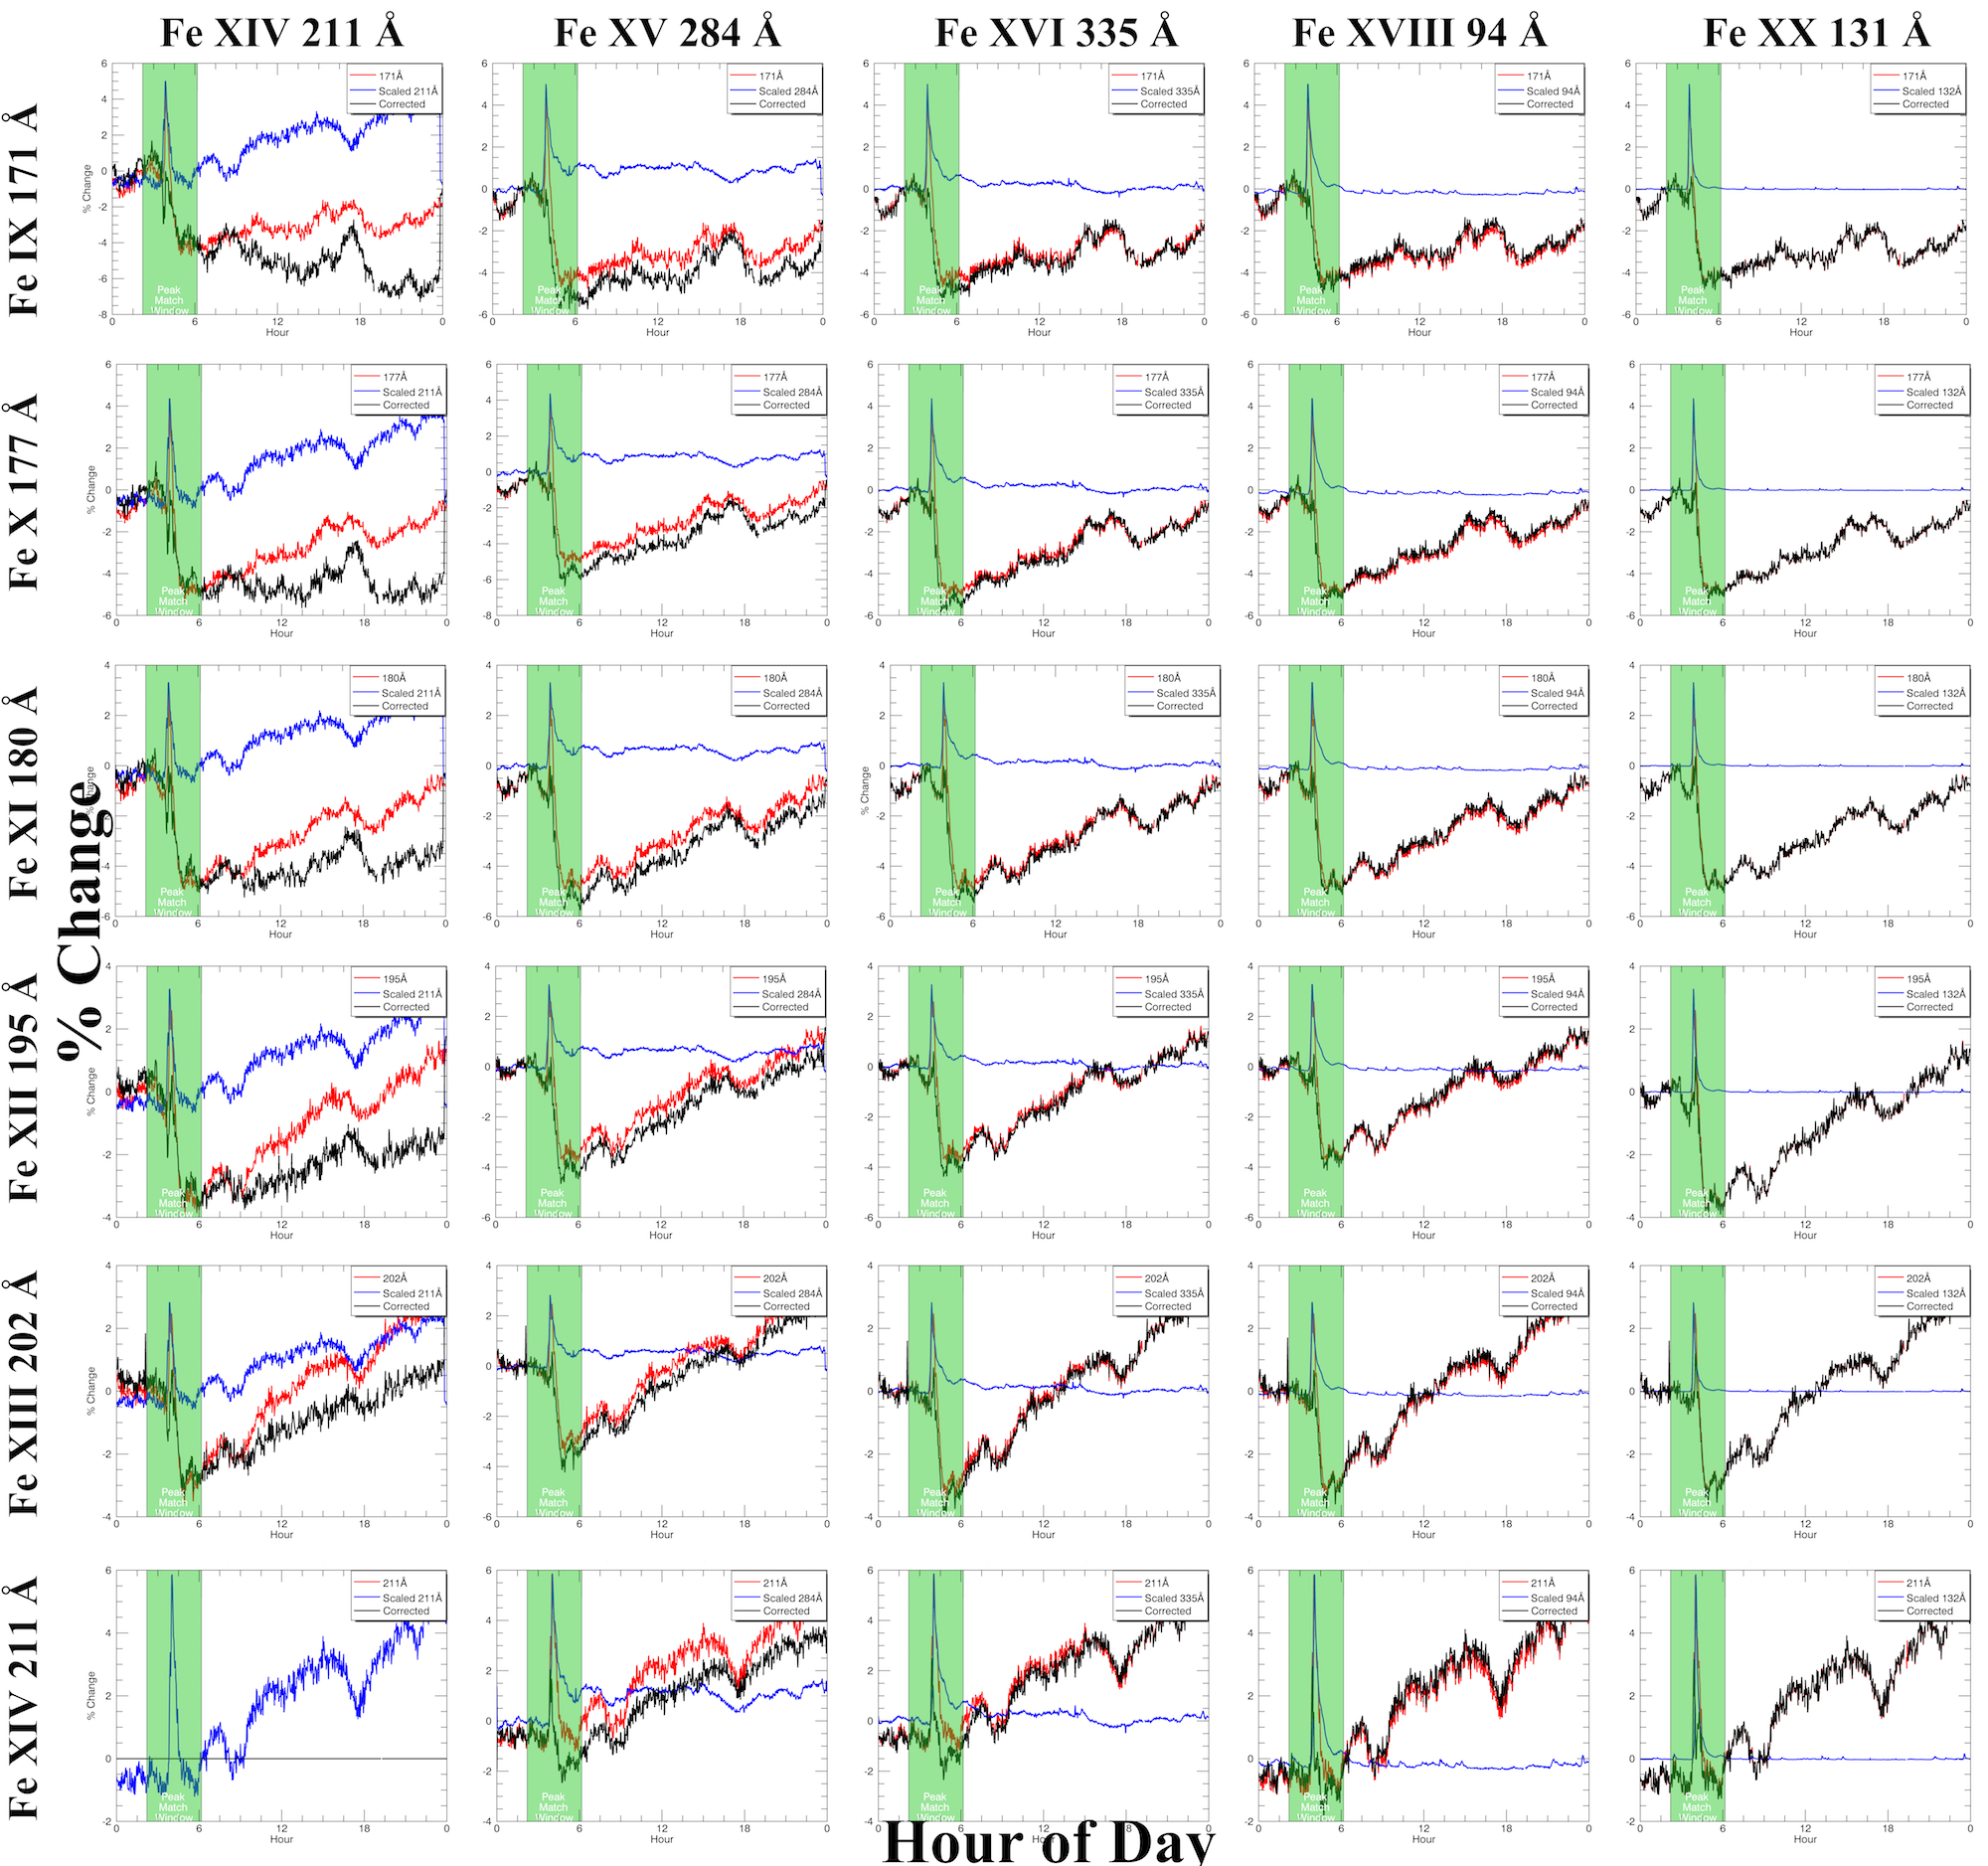
\includegraphics[width=\textwidth]{Images/AllDeconvolutionsEvent20.png}
    \end{center}
    \caption[All deconvolution combinations example]{
        Example of every combination of the dimming (rows) and nondimming (columns) lines for the deconvolution method for 
        a single event (Event 20). In each plot, the red is the dimming line, blue is the scaled and time shifted 
        nondimming line, and black is the result of the subtraction (red - blue). The vertical transparent green bar 
        indicates the time window the algorithm uses for finding and matching peaks. 
   	}
    \label{fig:deconvolutioncombinations}
\end{figure}

This methodology has been applied to the 28 unique EVE dimmings found during the four weeks studied. Of these, all 28 were found to be best represented by the 171 \AA\ - 284 \AA\ combination. It is possible that other coronal line pairings might be better for different spectral resolution measurements.

\section{Dimming Light Curve Fitting Method}
\label{sec:fittingmethod}

\subsection{Dimming Parameterization Method}
Include uncertainty derivations for depth/slope. Can consider making this a whole additional section instead of a subsection. If so, make sure to update introduction last paragraph. 

\section{Dimming and CME Parameters Correlation}
\label{sec:correlation}

\section{Summary} 
\label{sec:chapter5summary}








